% =========================================================================
% BÀI 07: HÌNH VUÔNG, HÌNH TRÒN, HÌNH TAM GIÁC, HÌNH CHỮ NHẬT (CHỦ ĐỀ 2)
% TOÀN BỘ CÂU HỎI ĐƯỢC VẼ HÌNH MINH HỌA TRỰC QUAN 100% BẰNG TIKZ
% =========================================================================

% =========================================================================
% PHẦN 1: TRẮC NGHIỆM LỰA CHỌN (12 CÂU)
% =========================================================================
\textbf{Phần 1. Trắc nghiệm lựa chọn (Học sinh quan sát hình và chọn đáp án đúng)}
\setcounterpageref{ex}{0}

% --- CÂU 1 ---
\begin{ex} %[1H2N07]
Hình nào dưới đây có dạng \textbf{hình tròn}?
\begin{center}
\setlength{\tabcolsep}{12pt}
\begin{tabular}{cccc}
  % A: Cửa sổ vuông
  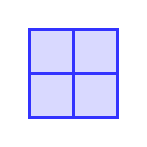
\begin{tikzpicture}[scale=0.7]
    \draw[fill=blue!15, draw=blue!80, line width=1.2pt] (-0.8,-0.8) rectangle (0.8,0.8);
    \draw[line width=1pt, blue!80] (0,-0.8) -- (0,0.8);
    \draw[line width=1pt, blue!80] (-0.8,0) -- (0.8,0);
  \end{tikzpicture}
  &
  % B: Đồng hồ tròn
  
\begin{tikzpicture}[scale=0.7]
    \draw[fill=orange!15, draw=orange!90!black, line width=1.3pt] (0,0) circle (0.85cm);
    \draw[fill=white, draw=orange!70] (0,0) circle (0.68cm);
    \foreach \a in {0, 30, ..., 330} {
      \fill[gray!80] (\a:0.56) circle (0.025cm);
    }
    \draw[line width=1.2pt, black] (0,0) -- (0,0.4);
    \draw[line width=1.4pt, red!80!black] (0,0) -- (0.3,0);
    \fill[black] (0,0) circle (0.05cm);
  \end{tikzpicture}
  &
  % C: Khăn quàng tam giác
  
\begin{tikzpicture}[scale=0.7]
    \fill[red!85!black] (-0.9,0.5) -- (0.9,0.5) -- (0,-0.6) -- cycle;
    \draw[line width=1pt, yellow!90!orange] (-0.8,0.42) -- (0.8,0.42) -- (0,-0.48) -- cycle;
  \end{tikzpicture}
  &
  % D: Hộp phấn chữ nhật
  \begin{tikzpicture}[scale=0.7]
    \draw[fill=teal!15, draw=teal!80!black, line width=1.2pt] (-1.1,-0.55) rectangle (1.1,0.55);
    \node[font=\tiny\bfseries\color{teal!90!black}] at (0,0) {HỘP PHẤN};
  \end{tikzpicture} \\[4pt]
  \textbf{A.} Cửa sổ & \textbf{B.} Mặt đồng hồ & \textbf{C.} Khăn quàng & \textbf{D.} Hộp phấn
\end{tabular}
\end{center}
\choice
{Cửa sổ}
{Khăn quàng đỏ}
{Hộp phấn}
{\True Mặt đồng hồ treo tường}
\loigiai{
Mặt đồng hồ có dạng hình tròn cong kín.\\
\textbf{Đáp án của câu hỏi là D}
}
\end{ex}

% --- CÂU 2 ---
\begin{ex} %[1H2N07]
Chiếc khăn quàng đỏ của bạn học sinh dưới đây có dạng hình gì?
\begin{center}
\begin{tikzpicture}[scale=0.85, baseline=(current bounding box.center)]
  \fill[red!85!black] (-1.8, 0.7) -- (1.8, 0.7) -- (0, -0.7) -- cycle;
  \draw[line width=1.3pt, red!60!black] (-1.8, 0.7) -- (1.8, 0.7) -- (0, -0.7) -- cycle;
  \node[draw=orange!80!black, fill=yellow!90, star, star points=5, star point ratio=2.2, line width=0.5pt, minimum size=0.55cm] at (0, 0.15) {};
\end{tikzpicture}
\end{center}
\choice
{Hình vuông}
{\True Hình tam giác}
{Hình chữ nhật}
{Hình tròn}
\loigiai{
Chiếc khăn quàng đỏ có 3 cạnh và 3 đỉnh, đó là \textbf{hình tam giác}.\\
\textbf{Đáp án của câu hỏi là B}
}
\end{ex}

% --- CÂU 3 ---
\begin{ex} %[1H2H07]
Chiếc bảng lớp học dưới đây có dạng hình gì?
\begin{center}
\begin{tikzpicture}[scale=0.85, baseline=(current bounding box.center)]
  % Khung gỗ ngoài
  \draw[fill=brown!40, draw=brown!80!black, line width=1.5pt, rounded corners=3pt] (-2.6,-1.0) rectangle (2.6,1.0);
  % Mặt bảng xanh lá đậm
  \draw[fill=green!45!black, draw=green!30!black, line width=1pt] (-2.3,-0.75) rectangle (2.3,0.75);
  % Đường kẻ phấn trắng mờ
  \draw[white!40, dashed, line width=0.5pt] (-2.1,0) -- (2.1,0);
  \node[font=\bfseries\color{white}] at (0, 0.25) {$1 + 2 = 3$};
  \node[font=\footnotesize\itshape\color{yellow!80}] at (0, -0.35) {Lớp 1A};
\end{tikzpicture}
\end{center}
\choice
{Hình tròn}
{\True Hình chữ nhật}
{Hình tam giác}
{Hình vuông}
\loigiai{
Mặt bảng có 2 cạnh dài và 2 cạnh ngắn, đó là \textbf{hình chữ nhật}.\\
\textbf{Đáp án của câu hỏi là B}
}
\end{ex}

% --- CÂU 4 ---
\begin{ex} %[1H2H07]
Viên gạch hoa lát nền nhà dưới đây có dạng hình gì?
\begin{center}
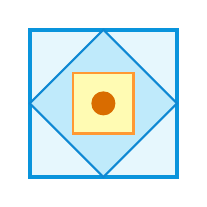
\begin{tikzpicture}[scale=0.85, baseline=(current bounding box.center)]
  \draw[fill=cyan!10, draw=cyan!80!blue, line width=1.5pt] (-1.1,-1.1) rectangle (1.1,1.1);
  \draw[fill=cyan!25, draw=cyan!70!blue, line width=0.8pt] (0,1.1) -- (1.1,0) -- (0,-1.1) -- (-1.1,0) -- cycle;
  \draw[fill=yellow!30, draw=orange!80, line width=0.8pt] (-0.45,-0.45) rectangle (0.45,0.45);
  \fill[orange!85!black] (0,0) circle (0.18cm);
\end{tikzpicture}
\end{center}
\choice
{Hình tam giác}
{Hình tròn}
{\True Hình vuông}
{Hình chữ nhật}
\loigiai{
Viên gạch hoa có 4 cạnh bằng nhau, đó là \textbf{hình vuông}.\\
\textbf{Đáp án của câu hỏi là C}
}
\end{ex}

\newpage
% --- CÂU 5 ---
\begin{ex} %[1H2H07]
Quan sát hình tam giác dưới đây. Em hãy đếm xem hình tam giác có bao nhiêu cạnh?
\begin{center}
\begin{tikzpicture}[scale=0.9, baseline=(current bounding box.center)]
  \draw[fill=orange!15, draw=orange!90!black, line width=1.6pt] (-1.6,-0.8) -- (1.6,-0.8) -- (0,1.2) -- cycle;
  % Đánh dấu 3 cạnh
  \node[font=\bfseries\color{red!85!black}] at (0, -1.15) {cạnh 1};
  \node[font=\bfseries\color{blue!80!black}, rotate=51] at (1.05, 0.4) {cạnh 2};
  \node[font=\bfseries\color{teal!80!black}, rotate=-51] at (-1.05, 0.4) {cạnh 3};
\end{tikzpicture}
\end{center}
\choice
{\True $3$ cạnh}
{$2$ cạnh}
{$4$ cạnh}
{$5$ cạnh}
\loigiai{
Hình tam giác có đúng \textbf{3 cạnh}.\\
\textbf{Đáp án của câu hỏi là A}
}
\end{ex}

% --- CÂU 6 ---
\begin{ex} %[1H2H07]
Quan sát hình vuông dưới đây. Hình vuông có bao nhiêu cạnh bằng nhau?
\begin{center}
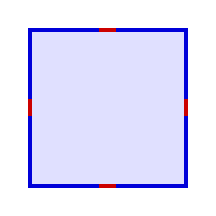
\begin{tikzpicture}[scale=0.9, baseline=(current bounding box.center)]
  \draw[fill=blue!12, draw=blue!85!black, line width=1.6pt] (-1.1,-1.1) rectangle (1.1,1.1);
  % Vạch đánh dấu 4 cạnh bằng nhau
  \draw[line width=1.5pt, red!80!black] (-0.12, 1.1) -- (0.12, 1.1);
  \draw[line width=1.5pt, red!80!black] (-0.12, -1.1) -- (0.12, -1.1);
  \draw[line width=1.5pt, red!80!black] (-1.1, -0.12) -- (-1.1, 0.12);
  \draw[line width=1.5pt, red!80!black] (1.1, -0.12) -- (1.1, 0.12);
\end{tikzpicture}
\end{center}
\choice
{$3$ cạnh}
{$2$ cạnh}
{$5$ cạnh}
{\True $4$ cạnh bằng nhau}
\loigiai{
Hình vuông có đúng \textbf{4 cạnh bằng nhau}.\\
\textbf{Đáp án của câu hỏi là D}
}
\end{ex}

% --- CÂU 7 ---
\begin{ex} %[1H2V07]
Biển báo giao thông hình tam giác dưới đây có bao nhiêu đỉnh (góc nhọn)?
\begin{center}

\begin{tikzpicture}[scale=0.85, baseline=(current bounding box.center)]
  \draw[fill=yellow!90!orange, draw=red!90!black, line width=2.5pt, rounded corners=3pt] (-1.5,-0.8) -- (1.5,-0.8) -- (0,1.4) -- cycle;
  % Dấu chấm than cảnh báo
  \fill[black] (-0.08,0.7) rectangle (0.08,0.05);
  \fill[black] (0,-0.25) circle (0.1cm);
  % Chấm tròn đánh dấu 3 đỉnh
  \fill[red!80!black] (0, 1.4) circle (0.12cm);
  \fill[red!80!black] (-1.5, -0.8) circle (0.12cm);
  \fill[red!80!black] (1.5, -0.8) circle (0.12cm);
\end{tikzpicture}
\end{center}
\choice
{\True $3$ đỉnh}
{$2$ đỉnh}
{$4$ đỉnh}
{$1$ đỉnh}
\loigiai{
Hình tam giác có \textbf{3 đỉnh} (3 góc nhọn).\\
\textbf{Đáp án của câu hỏi là A}
}
\end{ex}

% --- CÂU 8 ---
\begin{ex} %[1H2V07]
Cái đĩa đựng thức ăn tròn xoe dưới đây có dạng hình gì?
\begin{center}

\begin{tikzpicture}[scale=0.85, baseline=(current bounding box.center)]
  \draw[fill=teal!10, draw=teal!80!black, line width=1.5pt] (0,0) circle (1.2cm);
  \draw[fill=white, draw=teal!60, line width=1pt] (0,0) circle (0.85cm);
  \draw[fill=teal!20, draw=teal!50, line width=0.7pt] (0,0) circle (0.5cm);
\end{tikzpicture}
\end{center}
\choice
{Hình vuông}
{\True Hình tròn}
{Hình chữ nhật}
{Hình tam giác}
\loigiai{
Cái đĩa tròn có dạng \textbf{hình tròn}.\\
\textbf{Đáp án của câu hỏi là B}
}
\end{ex}

\newpage
% --- CÂU 9 ---
\begin{ex} %[1H2V07]
Quyển sách Toán 1 dưới đây có mặt bìa dạng hình gì?
\begin{center}
\begin{tikzpicture}[scale=0.85, baseline=(current bounding box.center)]
  \draw[fill=blue!15, draw=blue!85!black, line width=1.5pt, rounded corners=2pt] (-1.5,-1.4) rectangle (1.5,1.4);
  \draw[fill=yellow!40, draw=orange!80, line width=1pt] (-1.3,0.3) rectangle (1.3,1.1);
  \node[font=\bfseries\color{red!85!black}] at (0, 0.7) {TOÁN 1};
  \draw[fill=green!30, draw=green!70!black] (-1.0,-0.9) rectangle (1.0,-0.1);
  \node[font=\footnotesize\bfseries\color{green!80!black}] at (0, -0.5) {LỚP 1};
\end{tikzpicture}
\end{center}
\choice
{Hình tam giác}
{Hình tròn}
{Hình vuông}
{\True Hình chữ nhật}
\loigiai{
Bìa sách Toán 1 có dạng \textbf{hình chữ nhật}.\\
\textbf{Đáp án của câu hỏi là D}
}
\end{ex}

% --- CÂU 10 ---
\begin{ex} %[1H2V07]
Cắt đôi một hình vuông theo đường nét đứt (đường chéo), ta thu được 2 hình gì?
\begin{center}
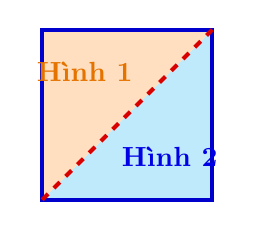
\begin{tikzpicture}[scale=0.9, baseline=(current bounding box.center)]
  % Nửa tam giác dưới
  \fill[cyan!25] (-1.2,-1.2) -- (1.2,-1.2) -- (1.2,1.2) -- cycle;
  % Nửa tam giác trên
  \fill[orange!25] (-1.2,-1.2) -- (-1.2,1.2) -- (1.2,1.2) -- cycle;
  \draw[line width=1.5pt, blue!80!black] (-1.2,-1.2) rectangle (1.2,1.2);
  % Đường chéo nét đứt
  \draw[line width=1.5pt, red!85!black, dashed] (-1.2,-1.2) -- (1.2,1.2);
  \node[font=\bfseries\color{orange!90!black}] at (-0.6, 0.6) {Hình 1};
  \node[font=\bfseries\color{blue!90!black}] at (0.6, -0.6) {Hình 2};
\end{tikzpicture}
\end{center}
\choice
{\True 2 hình tam giác}
{2 hình vuông}
{2 hình chữ nhật}
{2 hình tròn}
\loigiai{
Cắt chéo một hình vuông ta được \textbf{2 hình tam giác}.\\
\textbf{Đáp án của câu hỏi là A}
}
\end{ex}

% --- CÂU 11 ---
\begin{ex} %[1H2V07]
Ghép 2 hình tam giác bằng nhau lại như hình vẽ, ta tạo thành hình gì?
\begin{center}
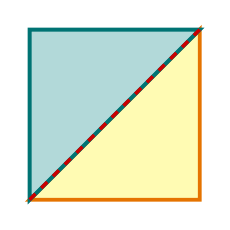
\begin{tikzpicture}[scale=0.9, baseline=(current bounding box.center)]
  % Tam giác 1
  \draw[fill=yellow!30, draw=orange!90!black, line width=1.4pt] (-1.2,-1.2) -- (1.2,-1.2) -- (1.2,1.2) -- cycle;
  % Tam giác 2
  \draw[fill=teal!30, draw=teal!90!black, line width=1.4pt] (-1.2,-1.2) -- (-1.2,1.2) -- (1.2,1.2) -- cycle;
  \draw[line width=1.2pt, red!80!black, dashed] (-1.2,-1.2) -- (1.2,1.2);
\end{tikzpicture}
\end{center}
\choice
{Hình tròn}
{Khối cầu}
{\True Hình vuông}
{Khối trụ}
\loigiai{
Ghép 2 hình tam giác vuông bằng nhau tạo thành \textbf{hình vuông}.\\
\textbf{Đáp án của câu hỏi là C}
}
\end{ex}

% --- CÂU 12 ---
\begin{ex} %[1H2C07]
Hình ngôi nhà dưới đây được ghép bởi mấy hình phẳng?
\begin{center}
\begin{tikzpicture}[scale=0.85, baseline=(current bounding box.center)]
  % Mái nhà tam giác
  \draw[fill=red!65!black, draw=red!90!black, line width=1.4pt] (-1.8, 0.6) -- (1.8, 0.6) -- (0, 1.8) -- cycle;
  \node[font=\footnotesize\bfseries\color{white}] at (0, 0.95) {Mái nhà};
  % Thân nhà hình vuông
  \draw[fill=yellow!35, draw=orange!80!black, line width=1.4pt] (-1.4, -1.0) rectangle (1.4, 0.6);
  \node[font=\footnotesize\bfseries\color{orange!90!black}] at (0, 0.25) {Thân nhà};
  % Cửa ra vào hình chữ nhật
  \draw[fill=cyan!35, draw=blue!80!black, line width=1.2pt] (-0.45, -1.0) rectangle (0.45, -0.15);
  \node[font=\tiny\bfseries\color{blue!90!black}] at (0, -0.6) {Cửa};
\end{tikzpicture}
\end{center}
\choice
{$2$ hình}
{$4$ hình}
{\True $3$ hình}
{$5$ hình}
\loigiai{
Gồm 3 hình phẳng: 1 hình tam giác (mái), 1 hình vuông (thân) và 1 hình chữ nhật (cửa).\\
\textbf{Đáp án của câu hỏi là C}
}
\end{ex}

\newpage
% =========================================================================
% PHẦN 2: TRẮC NGHIỆM ĐÚNG SAI
% =========================================================================
\textbf{Phần 2. Trắc nghiệm đúng sai (Quan sát hình vẽ và xét tính đúng/sai)}
\setcounterpageref{ex}{0}

% --- CÂU 13 ---
\begin{ex} %[1H2H07]
Quan sát 4 hình phẳng dưới đây:
\begin{center}
\setlength{\tabcolsep}{10pt}
\begin{tabular}{cccc}
  % Hình tròn
  
\begin{tikzpicture}[scale=0.65]
    \draw[fill=orange!25, draw=orange!90!black, line width=1.3pt] (0,0) circle (0.85cm);
    \node[font=\footnotesize\bfseries\color{orange!90!black}] at (0,-1.2) {Hình tròn};
  \end{tikzpicture}
  &
  % Hình tam giác
  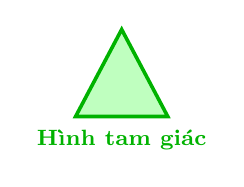
\begin{tikzpicture}[scale=0.65]
    \draw[fill=green!25, draw=green!70!black, line width=1.3pt] (-0.9,-0.75) -- (0.9,-0.75) -- (0,0.95) -- cycle;
    \node[font=\footnotesize\bfseries\color{green!70!black}] at (0,-1.2) {Hình tam giác};
  \end{tikzpicture}
  &
  % Hình vuông
  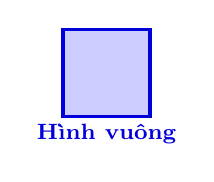
\begin{tikzpicture}[scale=0.65]
    \draw[fill=blue!20, draw=blue!85!black, line width=1.3pt] (-0.85,-0.85) rectangle (0.85,0.85);
    \node[font=\footnotesize\bfseries\color{blue!85!black}] at (0,-1.2) {Hình vuông};
  \end{tikzpicture}
  &
  % Hình chữ nhật
  \begin{tikzpicture}[scale=0.65]
    \draw[fill=purple!20, draw=purple!85!black, line width=1.3pt] (-1.1,-0.65) rectangle (1.1,0.65);
    \node[font=\footnotesize\bfseries\color{purple!85!black}] at (0,-1.2) {Hình chữ nhật};
  \end{tikzpicture}
\end{tabular}
\end{center}
Xét tính đúng sai của các câu sau:
\choiceTF
{\True Hình tròn có đường viền cong tròn khép kín}
{\True Hình tam giác có 3 cạnh và 3 đỉnh}
{Hình vuông có 3 cạnh bằng nhau}
{\True Hình vuông có 4 cạnh bằng nhau}
\loigiai{
\begin{itemize}
    \item Hình tròn là đường cong kín: \textbf{Đúng}.
    \item Hình tam giác có 3 cạnh và 3 đỉnh: \textbf{Đúng}.
    \item Hình vuông có 4 cạnh bằng nhau (nói 3 cạnh là sai): \textbf{Sai}.
    \item Hình vuông có 4 cạnh bằng nhau: \textbf{Đúng}.
\end{itemize}
}
\end{ex}

% --- CÂU 14 ---
\begin{ex} %[1H2V07]
Bạn Nam có bộ đồ chơi ghép hình gồm các hình phẳng dưới đây:
\begin{center}
\begin{tabular}{ccc}
  % 3 hình vuông
  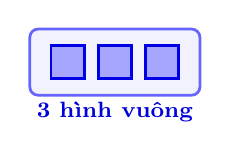
\begin{tikzpicture}[scale=0.6]
    \draw[fill=blue!5, draw=blue!60, line width=1pt, rounded corners=3pt] (-1.8,-0.7) rectangle (1.8,0.7);
    \foreach \x in {-1.0, 0, 1.0} {
      \draw[fill=blue!35, draw=blue!90!black, line width=1pt] (\x-0.35,-0.35) rectangle (\x+0.35,0.35);
    }
    \node[font=\footnotesize\bfseries\color{blue!85!black}] at (0,-1.05) {3 hình vuông};
  \end{tikzpicture}
  &
  % 2 hình tròn
  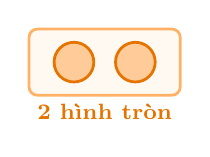
\begin{tikzpicture}[scale=0.6]
    \draw[fill=orange!5, draw=orange!60, line width=1pt, rounded corners=3pt] (-1.6,-0.7) rectangle (1.6,0.7);
    \foreach \x in {-0.65, 0.65} {
      \draw[fill=orange!40, draw=orange!90!black, line width=1pt] (\x,0) circle (0.42cm);
    }
    \node[font=\footnotesize\bfseries\color{orange!90!black}] at (0,-1.05) {2 hình tròn};
  \end{tikzpicture}
  &
  % 4 hình tam giác
  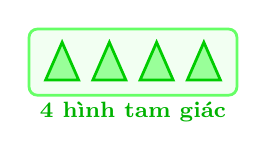
\begin{tikzpicture}[scale=0.6]
    \draw[fill=green!5, draw=green!60, line width=1pt, rounded corners=3pt] (-2.2,-0.7) rectangle (2.2,0.7);
    \foreach \x in {-1.5, -0.5, 0.5, 1.5} {
      \draw[fill=green!40, draw=green!80!black, line width=1pt] (\x-0.35,-0.38) -- (\x+0.35,-0.38) -- (\x,0.42) -- cycle;
    }
    \node[font=\footnotesize\bfseries\color{green!70!black}] at (0,-1.05) {4 hình tam giác};
  \end{tikzpicture}
\end{tabular}
\end{center}
Xét tính đúng sai của các câu sau:
\choiceTF
{\True Nam có nhiều hình tam giác nhất (4 hình)}
{\True Nam có ít hình tròn nhất (2 hình)}
{Nam có tất cả 10 hình phẳng}
{\True Nam có tất cả 9 hình phẳng ($3 + 2 + 4 = 9$)}
\loigiai{
\begin{itemize}
    \item Hình tam giác có 4 hình, nhiều nhất: \textbf{Đúng}.
    \item Hình tròn có 2 hình, ít nhất: \textbf{Đúng}.
    \item Tổng số hình là $3 + 2 + 4 = 9$ hình, nói 10 hình là: \textbf{Sai}.
    \item Tổng cộng có 9 hình: \textbf{Đúng}.
\end{itemize}
}
\end{ex}

% =========================================================================
% PHẦN 3: TRẢ LỜI NGẮN (ĐIỀN SỐ THÍCH HỢP)
% =========================================================================
\textbf{Phần 3. Trả lời ngắn (Quan sát hình vẽ và điền số thích hợp)}
\setcounterpageref{ex}{0}

% --- CÂU 15 ---
\begin{ex} %[1H2H07]
Em hãy đếm xem hình tam giác dưới đây có bao nhiêu cạnh?
\begin{center}
\begin{tikzpicture}[scale=0.85, baseline=(current bounding box.center)]
  \draw[fill=yellow!25, draw=orange!90!black, line width=1.6pt] (-1.6,-0.7) -- (1.6,-0.7) -- (0,1.2) -- cycle;
  \node[font=\bfseries\color{red!85!black}] at (0, -1.05) {Cạnh 1};
  \node[font=\bfseries\color{blue!80!black}, rotate=51] at (1.05, 0.45) {Cạnh 2};
  \node[font=\bfseries\color{teal!80!black}, rotate=-51] at (-1.05, 0.45) {Cạnh 3};
\end{tikzpicture}
\end{center}
\shortans{3}
\loigiai{
\textbf{Đáp số:} $3$\\
Hình tam giác có $3$ cạnh.
}
\end{ex}

% --- CÂU 16 ---
\begin{ex} %[1H2H07]
Em hãy đếm xem hình vuông dưới đây có bao nhiêu cạnh?
\begin{center}
\begin{tikzpicture}[scale=0.85, baseline=(current bounding box.center)]
  \draw[fill=cyan!20, draw=blue!85!black, line width=1.6pt] (-1.0,-1.0) rectangle (1.0,1.0);
  \node[font=\bfseries\color{red!85!black}] at (0, 1.35) {cạnh 1};
  \node[font=\bfseries\color{blue!80!black}] at (1.45, 0) {cạnh 2};
  \node[font=\bfseries\color{green!60!black}] at (0, -1.35) {cạnh 3};
  \node[font=\bfseries\color{orange!85!black}] at (-1.45, 0) {cạnh 4};
\end{tikzpicture}
\end{center}
\shortans{4}
\loigiai{
\textbf{Đáp số:} $4$\\
Hình vuông có $4$ cạnh bằng nhau.
}
\end{ex}

\newpage
% --- CÂU 17 ---
\begin{ex} %[1H2V07]
Quan sát chiếc xe đạp dưới đây. Có bao nhiêu chiếc bánh xe có dạng \textbf{hình tròn}?
\begin{center}
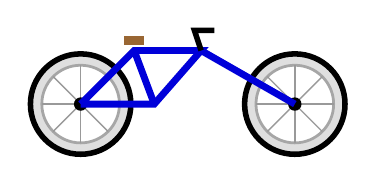
\begin{tikzpicture}[scale=0.85, baseline=(current bounding box.center)]
  % Bánh trước & bánh sau
  \foreach \bx in {-1.6, 1.6} {
    \draw[fill=gray!25, draw=black, line width=2pt] (\bx,0) circle (0.75cm);
    \draw[fill=white, draw=gray!70, line width=1pt] (\bx,0) circle (0.58cm);
    \foreach \ang in {0, 45, ..., 315} {
      \draw[line width=0.5pt, gray!80] (\bx,0) -- ++(\ang:0.58cm);
    }
    \fill[black] (\bx,0) circle (0.1cm);
  }
  % Khung xe đạp
  \draw[line width=2.5pt, blue!85!black] (-1.6,0) -- (-0.5,0) -- (0.2,0.8) -- (-0.8,0.8) -- (-1.6,0);
  \draw[line width=2.5pt, blue!85!black] (-0.5,0) -- (-0.8,0.8);
  \draw[line width=2.5pt, blue!85!black] (0.2,0.8) -- (1.6,0);
  % Ghi đông & Yên xe
  \draw[line width=2pt, black] (0.2,0.8) -- (0.1,1.1) -- (0.4,1.1);
  \draw[line width=3.5pt, brown!80!black] (-0.95,0.95) -- (-0.65,0.95);
\end{tikzpicture}
\end{center}
\shortans{2}
\loigiai{
\textbf{Đáp số:} $2$\\
Chiếc xe đạp có $2$ bánh xe hình tròn.
}
\end{ex}

% --- CÂU 18 ---
\begin{ex} %[1H2V07]
Quan sát chiếc thuyền buồm dưới đây. Đếm xem có bao nhiêu cánh buồm dạng \textbf{hình tam giác}?
\begin{center}

\begin{tikzpicture}[scale=0.85, baseline=(current bounding box.center)]
  % Mặt nước xanh
  \fill[cyan!12] (-2.4,-0.85) rectangle (2.4,-0.45);
  % Thân thuyền hình thang
  \draw[fill=brown!60!black, draw=brown!90!black, line width=1.5pt] (-1.8,-0.5) -- (1.8,-0.5) -- (1.2,-1.1) -- (-1.2,-1.1) -- cycle;
  % Cột buồm
  \draw[line width=2.5pt, brown!90!black] (0,-0.5) -- (0,1.5);
  % Cánh buồm lớn (tam giác phải)
  \draw[fill=red!70, draw=red!90!black, line width=1.2pt] (0.1,-0.3) -- (1.5,-0.3) -- (0.1,1.3) -- cycle;
  % Cánh buồm nhỏ (tam giác trái)
  \draw[fill=yellow!80, draw=orange!90!black, line width=1.2pt] (-0.1,-0.3) -- (-1.2,-0.3) -- (-0.1,1.0) -- cycle;
\end{tikzpicture}
\end{center}
\shortans{2}
\loigiai{
\textbf{Đáp số:} $2$\\
Có $2$ cánh buồm dạng hình tam giác.
}
\end{ex}

% --- CÂU 19 ---
\begin{ex} %[1H2V07]
Quan sát hình vẽ: có 4 hình vuông và 5 hình tam giác. Có tất cả bao nhiêu hình phẳng?
\begin{center}
\begin{tabular}{cc}
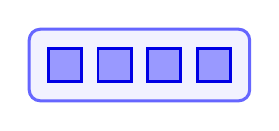
\begin{tikzpicture}[scale=0.7]
  \draw[fill=blue!5, draw=blue!60, line width=1.1pt, rounded corners=4pt] (-2.0,-0.65) rectangle (2.0,0.65);
  \foreach \x in {-1.35, -0.45, 0.45, 1.35} {
    \draw[fill=blue!40, draw=blue!90!black, line width=1pt] (\x-0.3,-0.3) rectangle (\x+0.3,0.3);
  }
\end{tikzpicture}
&
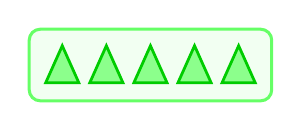
\begin{tikzpicture}[scale=0.7]
  \draw[fill=green!5, draw=green!60, line width=1.1pt, rounded corners=4pt] (-2.2,-0.65) rectangle (2.2,0.65);
  \foreach \x in {-1.6, -0.8, 0, 0.8, 1.6} {
    \draw[fill=green!45, draw=green!80!black, line width=1pt] (\x-0.3,-0.32) -- (\x+0.3,-0.32) -- (\x,0.35) -- cycle;
  }
\end{tikzpicture} \\[4pt]
{\bfseries\color{blue!85!black} 4 hình vuông} & {\bfseries\color{green!70!black} 5 hình tam giác}
\end{tabular}
\end{center}
\shortans{9}
\loigiai{
\textbf{Đáp số:} $9$\\
$4 + 5 = 9$ hình phẳng.
}
\end{ex}

% --- CÂU 20 ---
\begin{ex} %[1H2C07]
Mỗi hình vuông được ghép từ 2 hình tam giác. Để ghép thành 3 hình vuông như hình dưới đây, cần tất cả bao nhiêu hình tam giác?
\begin{center}
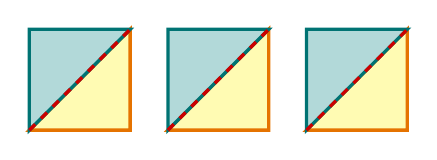
\begin{tikzpicture}[scale=0.8, baseline=(current bounding box.center)]
  \foreach \i in {0, 1, 2} {
    \draw[fill=yellow!30, draw=orange!90!black, line width=1.2pt] (\i*2.2-0.8,-0.8) -- (\i*2.2+0.8,-0.8) -- (\i*2.2+0.8,0.8) -- cycle;
    \draw[fill=teal!30, draw=teal!90!black, line width=1.2pt] (\i*2.2-0.8,-0.8) -- (\i*2.2-0.8,0.8) -- (\i*2.2+0.8,0.8) -- cycle;
    \draw[line width=1.2pt, red!80!black, dashed] (\i*2.2-0.8,-0.8) -- (\i*2.2+0.8,0.8);
  }
\end{tikzpicture}
\end{center}
\shortans{6}
\loigiai{
\textbf{Đáp số:} $6$\\
Có 3 hình vuông, mỗi hình cần 2 tam giác: $2 + 2 + 2 = 6$ hình tam giác.
}
\end{ex}
